% Chapter 4
%----------------------------------------------------------------------------------------
\section{A WSN with Waspmotes: Implementation aspects}
\subsection{Introduction}
\label{lab5}
In this section the program running on the WSN nodes will be discussed. To start programming, Libelium offers its customers a customized IDE\footnote{Integrated Development Environment (IDE)} and a fairly extensive API. The IDE uses the same compiler and core libraries as the Arduino IDE and is ideal to upload small examples and test programs to the nodes. However, to facilitate programming and to obtain more C/C++ support, expanding the API is required. This will be discussed in more detail in section \ref{LibAPI}.\\
After experimenting with the ZigBee sleep modes it became clear that the instability caused by delayed, pending messages for end devices could not be avoided. The program does support ZigBee sleep modes but this section will only discuss the \textit{stable operation modes without ZigBee sleep}. From now on, we will no longer differentiate between ZigBee routers and ZigBee end devices, but the sleep options will be controlled via Waspmote sleep modes, as recommended by Libelium \defcitealias{LIBSLEEP}{Libelium-dev, 2013}\citepalias{LIBSLEEP}. So a ZigBee router forced to sleep as well as a ZigBee end device will be considered an 'End Device'. 

%---------------------------------------------------

\subsection{Overall Program Structure}
\label{program}
When ZigBee sleep modes are ignored, basically three different programs suffice to program the entire network. There is one program to support the gateway (which is also the ZigBee coordinator) which analyses the data received from the other nodes, which is running on a Linux machine instead of a Waspmote. This will be discussed in section \ref{extracting}. All the nodes that collect sensor data are either running a 'Router' program or an 'End Device' program, which is designed to collect and send the sensor samples to the gateway. The only difference between these last two programs is that a 'Router' program does not implement sleep modes. The next sections will discuss the 'End Device' operation. A flowchart is shown in figure \ref{fig:flow}.\\
In a default program cycle each node has to associate with the network, measure some sensors, send the measured samples and possibly enter a sleep mode before repeating this cycle, depending on whether it has a 'Router' program or an 'End Device' program running.\\ 
\begin{table*}[htbp]
\begin{center}
\begin{tabular}[htbp]{|c|c|c|c|c|}
\hline
\textbf{Mode} & \textbf{Consumption} & \textbf{CPU} & \textbf{Cycle} & \textbf{Accepted Interruptions}\\
\hline
ON & 9mA & ON & - & Synch and Asynch\\
\hline
Sleep & 62$\mu$A  & ON & 31ms - 8s & Synch (WDT) and Asynch\\
\hline
Deep Sleep & 62$\mu$A & ON & 8s - min/hours/days & Synch (RTC) and Asynch\\
\hline
Hibernate & 0.7$\mu$A & OFF & 8s - min/hours/days & Synch (RTC)\\
\hline
\end{tabular}
\caption{The operational modes of Libelium Waspmote V1.1}
\label{tab:cons1}
\end{center}
\end{table*}
\begin{figure*}[htbp]
\centering
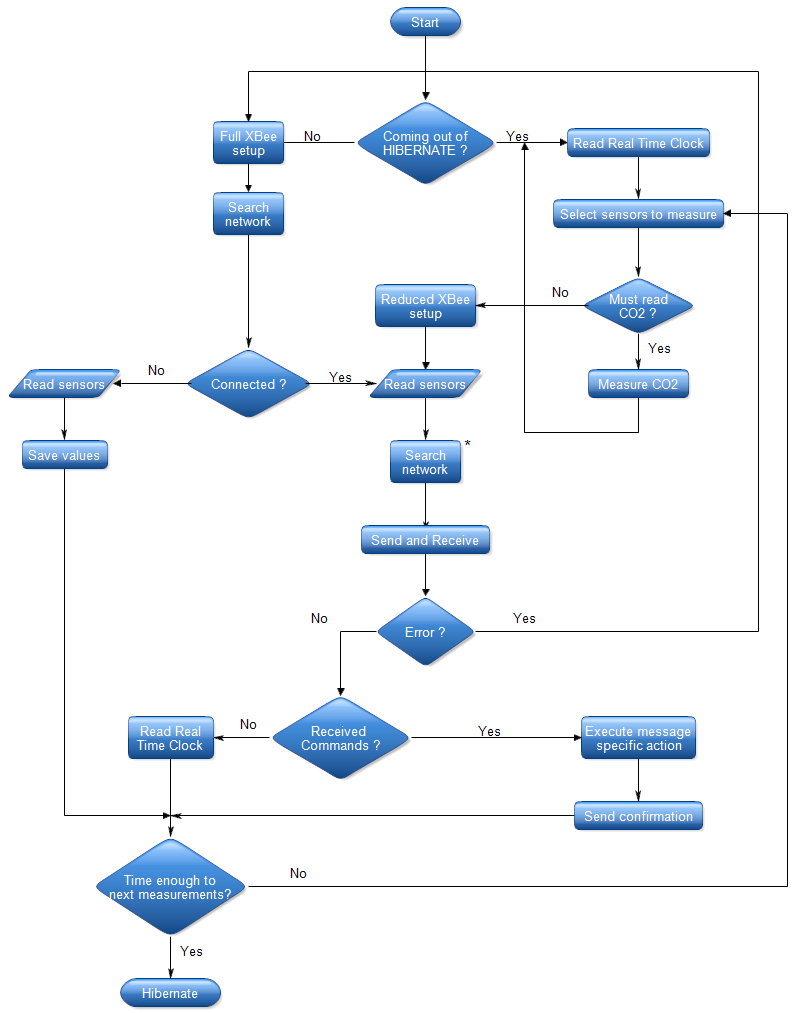
\includegraphics[height=19cm]{WSN2}
\caption{A flow chart of the Waspmote program for end devices}
\label{fig:flow}
\end{figure*}

\subsubsection{Initialization}
\label{initial}
\paragraph{Device start-up: Full initialization}
When the program is executed for the first time, a full XBee setup will be executed with the parameters retrieved from the program in the Libelium IDE. To ensure stability it takes about 8 seconds to write the settings to the XBee, to reset it afterwards (turn the power off and back on) and finally to perform the joining process. From this moment on the node will send its battery level to the coordinator and wait to receive an 'ADD\_NODE\_REQUEST' packet, containing its physical sensor layout settings, from the web interface. Until such a packet is received the node's sleeping time will gradually be increased.
\paragraph{Next cycles: Reduced initialization}
By not resetting the PAN ID but simply fetching it from the XBee's memory, the joining process only takes about two seconds\footnote{By enabling ZigBee sleep, the node does not lose the association with its parent and the re-joining process only takes about 10ms. However, the time needed to receive messages pending in router devices varies between 5 and 15 seconds and is never compensated by the faster joining process. There is also no guarantee that pending messages will be received or in which order they will be received, so network stability can no longer be guaranteed.} (Please see appendix \ref{timess} for more measurement results). Unfortunately a disadvantage of this shortened setup is that the XBee is no longer able to detect if the coordinator or his parent is actually available. The result of the executed association check is not always correct and the program will only notice this for the first time when it is trying to send a message. If this function results in a send error the program will do a full setup routine and resend the message. If the node then fails again to send the message we can conclude that the coordinator is really off-line or that there are no joinable nodes within range. In that case the message content will be saved and tried to be sent during the next cycles. In order not to lose the results, the gateway or web interface can keep track of the number of consecutive cycles a node has failed to report and notify a system administrator to avoid losing the saved values.

\subsubsection{Measuring sensors}
To sample a sensor from the expansion board, the Libelium API functions can be used. The functions return a float value corresponding to the sensor's measuring unit. Until an 'ADD\_NODE\_REQUEST' is received each node will measure its battery level and send it to the gateway. Via this packet the node gets to know its physical sensor layout and can decide if a future request of a sensor value is allowed.\\
%------------------------------
%\paragraph{Sample conversion}
To shorten messages (the ZigBee maximum payload is 74 Bytes \defcitealias{ZBGUIDE}{Waspmote ZigBee Networking Guide, 2012}\citepalias{ZBGUIDE} ) and to reduce transmission times, all values are sent in hexadecimal representation. This way all sensors fit within with 1 or 2 bytes. An example conversion is given for a temperature sample with two decimals:
\usestyle{vs} %other useful styles are, bw,  borland, vs
\includecode{tempConv.cpp}
%------------------------------

\subsubsection{Sending samples}
\label{frames1}
The API of Waspmote V1.1 introduces an 'Application Header' (see figure \ref{fig:appH} ) to send and receive data. This header takes care of packet fragmentation if packets exceed the maximum payload limit and can also be used by the receiver to treat the packet or fragment. The header itself is sent inside the RF Data field of the API Frame Structure, which was discussed in more detail in section \ref{ZBStructure} (see figure \ref{fig:frames}).
\begin{figure}[ht]
\centering
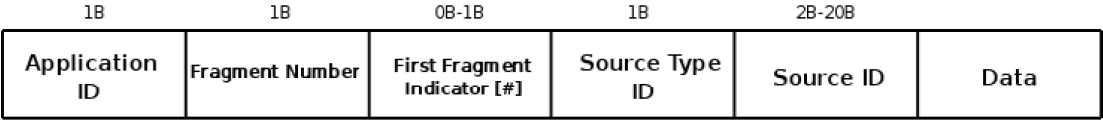
\includegraphics[width=0.48\textwidth]{appHeader}
\caption{The application Header}
\label{fig:appH}
\end{figure}\\
\noindent
The Waspmote and gateway programs use the 'Application ID' field in this header to distinguish different data packets. This extra layer also serves as an acknowledgement in the communication protocol. Depending on the 'Application ID' the layer contains a sensor mask (a 16 bit-flag) and data. With uniform timing settings, when a node awakens, it will measure the sensors found in its 'activeSensorMask' and send them to the gateway via an 'IO\_DATA' packet. This packet will be indicated as 'IO\_DATA' via the 'Application ID' field and will contain the mask of the measured sensors followed by their corresponding values.\\
To easily process this mask all sensor types are stored as follows:
\usestyle{vs} %other useful styles are, bw,  borland, vs
% Include the source code 
\includecode{sensType.cpp}
The sensor mask of a packet as well as the active mask stored in a certain node is a 16-bit value in which each bit indicates if a sensor must be taken into account or not.

%------------------------------
\paragraph{Escaping zeros}
Before sending the hexadecimal values all zeros must be removed (zeros are interpreted as end of string characters). Zeros will be replaced by \verb+0xFFFE+, so an extra byte is necessary. \verb+0xFF+ is the chosen escape character and \verb+0xFE+ is added to distinguish between an escaped zero and the value \verb+0xFF+ itself. The escaped character itself is of course also escaped.
\paragraph{Constructing packets}
To easily introduce the sensors into the packet to be sent, the program uses static function pointers. Part of the code to insert the measured sensors into an 'IO\_DATA' packet is given below. All Waspmote functions with error checking start with \verb+uint8_t error = 2+. If the returned error equals 2, the function has not been executed. Whereas 1 means something went wrong and 0 indicates a success. Each function pointer knows the size of the sample and updates the \verb+pos+ variable, which determines the location of the sample in the 'IO\_DATA' packet. This size and thus position depends on which sensor is included into the packet. The first two bytes of this packet are reserved for the sensor mask, indicating which sensor values are following. For example, an 'IO\_DATA' packet with as mask \verb+0x09+ indicates to the gateway that the packet contains temperature and battery data.
\usestyle{vs} %other useful styles are, bw,  borland, vs
% Include the source code 
\includecode{fp.cpp}
%------------------------------
\subsubsection{Wait for received messages}
To assure overall stability ZigBee sleep (see appendix \ref{zigbeesleep}) is not used, meaning nodes can only receive messages when they are turned on. To coordinate this, the end devices will check all messages for a fixed amount of time immediately after sensor data has been sent. It allows the gateway to send all its pending messages for this node. This means the Waspmote will only wake up when sensors have to be measured.\\
To select the right function when a request packet is received, the program uses function pointers in the same way it adds data to packets. There are a few additions however. Firstly a check is done if the received Packet ID is a valid index in the array of function pointers. This way, when intruders send an invalid Packet ID, the program will not crash because it jumped to a wrong place in program memory. Secondly the node will check if the sending node is authorized by comparing the origin's MAC address in the API frame to its authorized nodes. By default, only the gateway XBee radio is authorized.
For example, when an 'ADD\_NODE\_REQ' is received, some settings will be done and the node will send either an 'ADD\_NODE\_RES' or an 'SEND\_ERROR' packet back to the gateway. Appendix \ref{OwnProtocolLabel} shows a complete overview off all the Application IDs stored in the following enum:
\usestyle{vs} %other useful styles are, bw,  borland, vs
\includecode{appID.cpp}
%------------------------------
\subsubsection{Enter low power mode}
The user can set the device role ('Router' or 'End device'\footnote{This affects the Waspmote sleep mode. Setting 'Coordinator' role or changing the ZigBee device role is not possible because the XBee radio must be reflashed for this (The XBee's memory is to small to contain all profiles at the same time)}) during setup or even later on by sending a command to the Waspmote, which makes it easy to change a mote's device role. The device role is stored in the xbeeZB device type identifier (see \defcitealias{ZBGUIDE}{Waspmote ZigBee Networking Guide, 2012}\citepalias{ZBGUIDE} and '\textbf{WaspXBeeZBNode.h}').\\ 
Several Waspmote sleep functions have been added to the Libelium API, the most advanced one combines \textit{Sleep} and \textit{Hibernate} depending on the duration of the next time to sleep. By doing this the number of EEPROM writes is minimized. In one of the sleep modes, the program is paused and the next time to wake can be fetched from SRAM memory. With hibernate however, the node is completely disconnected from the main battery and all program variables are lost, so they must either be stored in the onboard EEPROM memory or on the optional micro-SD card. To save the scarce free memory and to optimize power consumption the EEPROM option is chosen and the objects needed to control the SD-card have been removed from the API.\\
As indicated in table \ref{tab:cons1}, only \textit{Deepsleep} and \textit{Hibernate} make use of the Waspmote's RTC, which is perfect to set the time to wake up and to select the sensors to measure. Unfortunately it is not possible to combine RTC usage for both \textit{Hibernate} and \textit{Deepsleep}, from the moment \textit{Hibernate} is implemented the RTC can no longer be used for other functionalities. So a tweak has been implemented to use the Watchdog instead, making it possible to combine \textit{Hibernate} and \textit{Sleep}.\\
To determine the next time to sleep several algorithms can be used, depending on the used Waspmote sleep mode. Since we are working with embedded systems with limited possibilities, one should also consider to limit the users options in order to facilitate the calculations. When the program detects inefficient measuring intervals, for example, 1 minute and 2 minutes 10 seconds, this can be notified to the installer or even be refused during setup.Another one of those limitations is a maximum of 10 seconds time resolution, meaning each value in the algorithm must be multiplied by 10. Suppose we want to measure one sensor each 30 seconds, another one each 40 seconds and a last one every 100 seconds. This means the node has to wake up at each multiple of those measuring intervals. The absolute times to wake up will be at\verb+ 0 3 4 6 9 10 12 15 18 20 21 24 27 28+. Each time the Waspmote wakes up, it will compare its current RTC value with the stored times. The biggest stored time that is an integer multiple of the RTC value is the current position in the array. With this time we can determine which sensors to measure and what the next time to sleep will be. The shortest algorithm to calculate these values is given below. From the moment the calculated times reach the least common divider (LCM) of the measuring intervals the algorithm can stop. Recursion is nice, however, without compiler optimization this is not recommended for embedded devices. To execute the code literary we would need extra instructions and memory for each function call\footnote{Each call requires a stack frame, containing the function parameters, return address and possibly local variables.}, which can easily lead to stack overflows in case of embedded devices. Since this algorithm is tail recursive the recursive calls can simply be replaced by a loop, eliminating the overhead\footnote{GCC with O3 optimization recognizes tail recursion and will do this for us}.
\usestyle{vs} %other useful styles are, bw,  borland, vs
\includecode{recursive.cpp}
%---------------------------------------
\subsubsection{Router program}
The 'Router program' is based on the same concepts discussed in the previous subsections, which were describing 'End Device' operation. The main difference is that a router node will not implement sleep possibilities and attention will be divided differently.\\
A 'Router program' will continuously check for new requests and will be interrupted by the RTC when it has to measure and send sensors. Initialization, measurements and sending samples is the same as for end devices.

%---------------------------------------------------------------------------------

\subsection{Weather Station Program}

Although the previous section stated there are only two different program versions running on the mobile nodes, this section will briefly discuss one more variant. The program running on the weather station, installed on the roof of Group T Campus Vesalius (see figure \ref{fig:weather}), is actually a specialized version of an 'End Device' program.\\
Firstly, because the weather station is equipped with a solar panel for energy harvesting, enabling the hibernate interruptions to save power consumption is no longer required. This means the RTC interruptions are fully available to determine the sampling intervals.\\
The weather station Waspmote is also equipped with an 'Agriculture Sensor Board' instead of a 'Gasses Sensor Board'. This means, for example, to sample the temperature sensor, different API functions must be used. Unfortunately, when the program creates both those objects (see section \ref{object}), none of the sensor readings are  correct any more. To solve this and to save program memory at the same time, conditional pre-processor directives are used. To compile for the weather station node, \verb+#define WEATHER_STATION+ must be uncommented in 'BjornClasses.h'.\\
The weather station program also has an extra interrupt routine attached. This interrupt is triggered each time the pluvio meter becomes full, incrementing the pluvio counter. When this happens for the first time within one hour, a started raining notification will be sent to the gateway. Afterwards, the pluvio meter counter can be read to know the millimetres of rainfall since the first interrupt occurred.\\
\begin{figure}[t]
\centering
\includegraphics[width=0.48\textwidth]{weather}
\caption{The weather station deployed on the roof of Group T, campus Vesalius}
\label{fig:weather}
\end{figure}
%According to Libelium their IDE has been properly tested and proven to assure optimum operation. Unfortunately we cannot agree with this. 
%Libelium also offers a lot of program examples on their website. Sadly most of them don't work like Libelium claims they do.
\begin{figure}[H]%[!h]
\centering
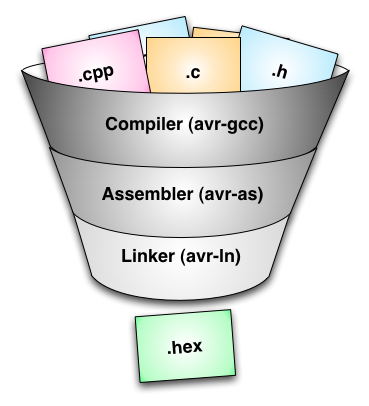
\includegraphics[width=0.26\textwidth]{avr}
\caption{An overview of the AVR toolchain}
\label{fig:tool}
\end{figure}
\begin{figure}[H]
\centering
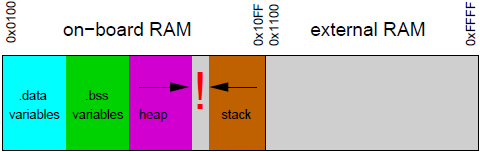
\includegraphics[width=0.48\textwidth]{ram}
\caption{The AVR / ATmega1281 standard RAM layout}
\label{fig:RAM}
\end{figure}
\subsection{AVR compiler}
\subsubsection{Toolchain Overview}
To develop software for an AVR microcontroller several tools are working together. This group of tools produces the final executable and is commonly called a toolchain and is shown in figure \ref{fig:tool}. 
\paragraph{GCC:} AVR uses the open source GNU Compiler Collection (GCC) with AVR microcontroller as target system. This version of GCC is known as 'AVR GCC' \defcitealias{AVR}{AVR-Libc User Manual, 2008}\citepalias{AVR}. GCC differs from other compilers, it only focuses on translating high level language to target assembly. For AVR GCC there are 3 language options: C, C++ and Ada. 
\paragraph{GNU Binutils: }The next step is done by another open source project called GNU Binutils. This contains the GNU assembler and GNU linker.
\paragraph{AVR-libc:} GCC and Binutils provide the tools to make the machine code but one critical component they do not provide is the Standard C Library. The open source AVR toolchain therefore comes with its own open source C Library project which contains many of the same functions found in the regular Standard C Library. It also adds many additional library functions that are specific to  AVR microcontrollers.
\paragraph{GNU Make:} Finally all pieces must be tied together. This is done by Make, which interprets and executes the Makefile of the project.
%------------------------------
\subsubsection{Memory Sections}
\label{memory}
The available non-volatile memory sections are the \textbf{.text} section (FLASH), which contains the actual machine instructions and the \textbf{.eeprom} section. Many AVR devices have a minimal amount of RAM. This limited amount of runtime memory needs to be shared between the following memory sections:
\begin{enumerate}
\item All initialized variables and static data such as\\ \verb+char message[] = "An error message"+ or \verb+USB.println("Another message")+ are stored in \textbf{.data variables}
\item Uninitialized global or static variables: \textbf{.bss variables}
\item Dynamic memory: \textbf{heap}
\item Area used for calling subroutines and storing local variables: \textbf{stack}
\end{enumerate}
The standard RAM layout is shown in figure \ref{fig:RAM}. Since there is no hardware supported memory management, separate regions can overwrite each other. Heap and stack can collide if either of them require large memory space or even when the allocations aren't high at all but because heap allocations get fragmented over time and new request don't fit in freed areas.\\ %figure was here
As discussed in section \ref{memory} the ATmega1281 is uses a modified Harvard architecture, meaning that data can also be stored in program memory space. This is useful when you have constant data and you're running out of room to store it. Remember that many AVRs have limit amount of RAM to store data, but may have available FLASH space left. For the compiler this is however a challenge, which is exacerbated by the fact that the C Language was designed for Von Neumann architectures. So the AVR compiler has to use other means to operate with these separate address spaces (cf. pointer usage). The AVR toolset used the GCC \verb+__attribute__+ keyword, which is used to attach different attributes to function declarations and variables. AVR GCC provides a special attribute called \verb+progmem+ for data declarations and tells the compiler to store the data in Program Memory. To increase the convenience to the end user AVR-libc provides a simple macro \verb+PROGMEM+ which can be found in 'avr/pgmspace.h'. To read the data another macro is provided, which generates the correct address to retrieve the data from Program Memory. Storing data in Program Space incurs extra overhead in terms of instructions and execution time, but usually this is minimal compared to the space savings.\\
\subsubsection{Memory problems}
Libelium's Programming Style Guide warns its users about the amount of memory \verb+USB.print("Test message!")+ requires. The program memory increases due to the instructions and arguments (the chars) needed to print the string. Since also the message itself is stored in the \textbf{.data} section \defcitealias{AVR}{AVR-Libc User Manual, 2008}\citepalias{AVR}, precious memory is wasted. As a fix, Libelium recommends to do the following:
\usestyle{vs}
\includecode{mem1.cpp}
This however still uses both program and data memory and is only useful if one wants to print the same message in different parts of the program, so this is not really a solution. The only way to save RAM memory while printing messages is to hard code them on the stack by doing the following:
\usestyle{vs} 
\includecode{mem2.cpp}
A less cumbersome way would be to give the message and an address where to store the message as argument of a recursive macro which does this operation for us. However, standard C macros cannot simply split a string into characters. So the only ways to save RAM is to hard code the string as data or to store the string in Program Space and use the \verb+strcpy_P+ to copy the string to stack when it is needed. 
\subsubsection{Compiler bugs}
When combining all pieces of software discussed in section \ref{program}, the Waspmote failed after a few cycles. It appeared as if Libelium's \verb+sendXBee(packetXBee *)+ function had a constant memory leak of 302 bytes. However, after examining all the related functions it became clear there were no implementation errors. After putting the necessary \verb+USB.print(freeMemory())+ statements before and after \verb+free()+ instructions, we concluded the \verb+free()+ instruction at line 5252 of 'WaspXBeeCore.cpp' failed\footnote{Issue 857: avr-libc 1.6.4 dynamic memory (malloc, free) bug, available at \url{https://code.google.com/p/arduino/issues/detail?id=857}, confirms this conclusion}. This was avoided by introducing a stack variable instead of a heap variable.\\
Another bug we discovered is with the assignment operator. For example assigning a \verb+uint16_t+ stack variable, that was needed for some evaluation, to a global \verb+uint16_t+ variable also fails sometimes for no clear reasons. Instead of using the temporarily stack variable, we re-assigned the evaluation to the global variable.    

\subsection{Libelium IDE and API}
\subsubsection{Waspmote-IDE}
The Libelium IDE offers some advantages compared to using other IDE's. For example by using Eclipse it is possible to update programs that are to big thereby over-writing the bootloader. Then they must be sent back to Libelium to restore them. The Waspmote IDE does not allow this accident, so Libelium does not support using other IDE's in an official way so that there is no valid warranty if you've erased the bootloader.\\
%------------------------------------
\subsubsection{Waspmote-API}
\label{LibAPI}
To facilitate the programming Libelium offers a quite big API and after some exploring you are quickly started with it. The structure of the API is very simple, there is little to no inheritance\footnote{Have a look at the graphs available at \url{http://www.libelium.com/v11-files/api/waspmote/db/d09/WaspClasses_8h.html} to get a complete overview of the API structure}. In this section, the most important classes are indicated with a red box and are recommended to explore before starting future programming.
\begin{figure*}[htbp]
\centering
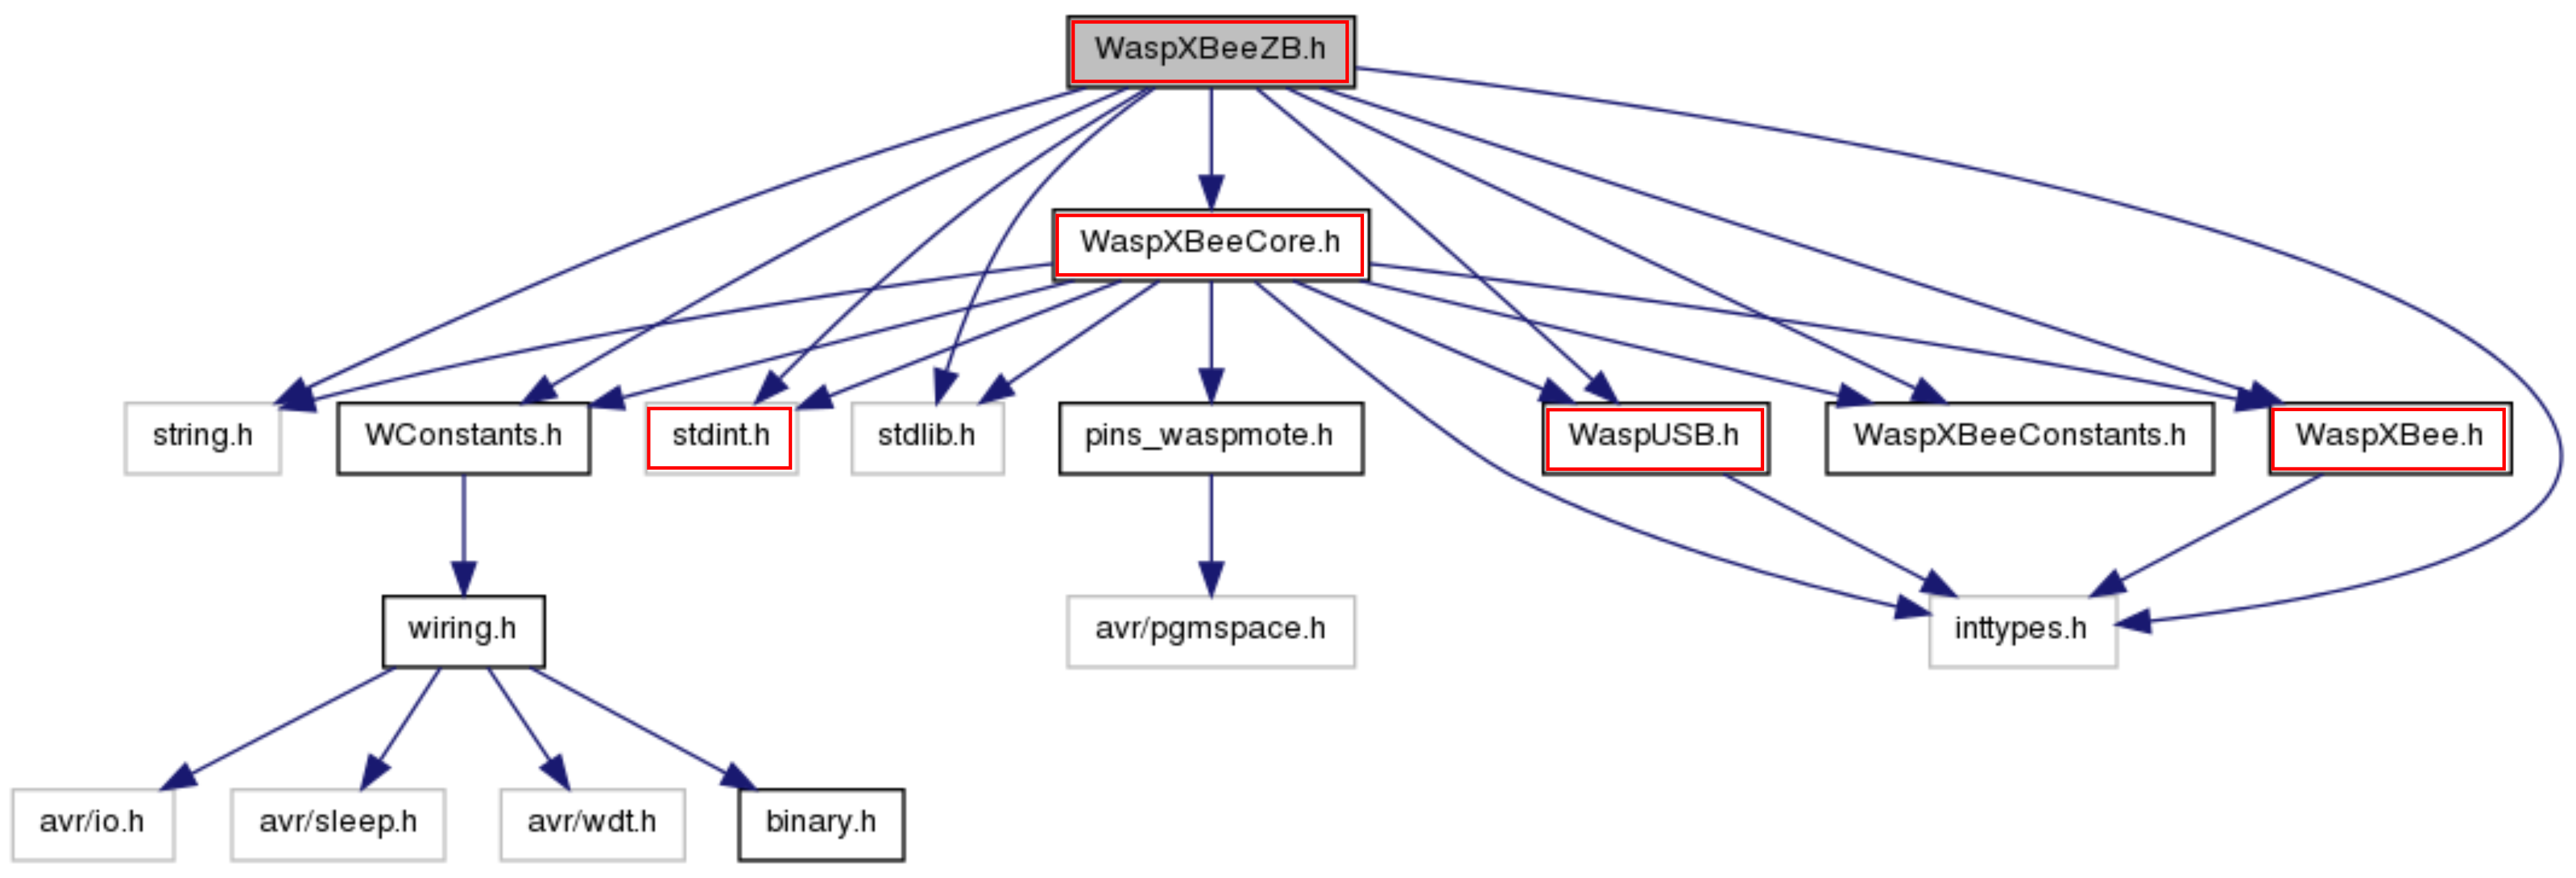
\includegraphics[width=0.98\textwidth]{API2}
\caption{Reduced dependency of Waspmote core libraries}
\label{fig:API2}
\end{figure*}
\paragraph{Original structure}
\label{object}
Each module or concept has its own class, for example all RTC functions are in 'WaspRTC.h' and 'WaspRTC.cpp'. To be able to use those functions in the IDE an object from the class 'WaspRTC' must be created. This object is created by default by the library and it is public to all libraries. All types to be run on the API can be found in the 'WaspClasses.h' file and each file also includes this file so it is aware of all available types.\\
For our application WaspXBeeZB is one of the most important classes. It inherits from WaspXBee Core and this way it is also related to the WaspXBee class. Figure \ref{fig:API2} displays the relationship with the AVR-libc libraries and the Waspmote hardware.\\ 
During the development of our program the Waspmote showed several strange effects that could only be explained by bad stack management or heap and stack conflicts. Because of this lack of free memory (SRAM, 8KB) we discovered that the V1.1 API wastes a lot of memory by always including all libraries, despite not using them. As a fix Libelium recommends via their forum to remove all classes you do not use, including there fields that are used in other classes, 'just' going through all the compiler errors one by one. After doing this our program had enough free memory and showed normal behaviour again.
%------------------------------------
\paragraph{Added functionality}
To facilitate programming extra functionality has been added to the Libelium API. They are inside files containing the original name with the 'Utils' addition, for example 'WaspRTCUtils.h' and can be found in 'BjornClasses.h'.
